%
% Modellbildung
%
% @version 1.0
% @author dmayer
% @created 29. Dezember 2015

\setchapterpreamble[o]{%
\dictum[--- \textsc{Norbert Wiener}, \emph{US-amerikanischer Mathematiker}]{\Gun Das beste Modell für eine Katze ist eine Katze; möglichst dieselbe Katze. \Gob}}
\renewcommand{\chapterheadstartvskip}{\vspace*{2cm}}

\chapter{Modellbildung und Simulation}
\label{chap:modellbildung}

Ziel dieses Kapitels ist es, ein hinreichend exaktes Modell zur Berechnung der Raumtemperatur in K004b zu bilden. Die Modellbildung soll physikalisch motiviert sein und daher auf den thermodynamischen Prozessen mit der Außenumgebung und der Anlage aus Kapitel \ref{chap:anlagendesign} basieren. Des Weiteren soll das Modell speziellen Anforderungen genügen, um eine Modellprädiktive Regelung der Anlage zu ermöglichen.

Dazu wird zunächst ein einfaches Grundmodell für einen hypothetischen Raum gebildet, dass anschließend schrittweise an den bestehenden Raum erweitert angepasst wird, bis eine die Qualität/Güte des Modells ausreichend ist.

\section{Modellbildung}

\subsection{Anforderungen an das Raummodell}
Die triviale Aufgabe des Modells ist eine hinreichend genaue Beschreibung der realen Vorgänge und des Temperaturverlaufs. Hinreichend bedeutet, dass das Modell eine ausreichende Güte für den Einsatz mit Modellprädiktiver Regelung besitzt. In Kapitel \ref{sec:mpc} wurden bereits die Grundlagen zur Modellprädiktiven Regelung erläutert, wodurch sich Einschränkungen bei der Modellbildung ergeben. Dabei wurde festgestellt, dass die Lösung von Optimalsteuerungsproblemen gradientenbasiert erfolgt und die zweifache Erzeugung von Ableitung erfordert. Damit ergibt sich die Anforderung, dass das Modell keine Unstetigkeiten aufweist und sich zweimal stetig differenzieren lässt.
Zudem ist Berechnung von Lösungen für Optimalsteuerungsprobleme sehr rechenintensiv und muss während des laufenden Betriebs der Anlage wiederholt stattfinden. Da die Lösung zudem wiederholt stattfinden muss
, wird eine erhöhte Rechenkapazität benötigt, 
um die Lösung in ausreichender Zeit zu berechnen. 

Daraus ergibt sich eine weitere Anforderung, denn um den Rechenbedarf möglichst gering zu halten, soll das Modell möglichst wenig KOmplexität besitzen.
Wie bereits bei den Anforderungen an die Anlage in Abschnitt \ref{sec:anforderungen} festgestellt wurde, stellt die Umgebung zur Optimalsteuerung einen begrenzenden Faktor dar, wodurch das Modell mit der Modellierungssprache Modelica gebildet wird.

Da diese Anforderungen teils gegenläufig sind, gilt es einen Kompromiss zu finden, ein stetig differenzierbares Modell,
, um eine ausreichende Modellgüte zu erhalten, gleichzeitig jedoch keine hohe Komplexität oder einen großen Umfang an Gleichungen besitzt.
Ziel: Hohe Modellgüte bei gleichzeitig geringer Komplexität und Stetigkeit

Daher wird im Folgenden zunächst ein simples Raummodell gebildet, dass anschließend sukzessive erweitert und damit die Komplexität des Modells schrittweise erhöht wird, bis eine ausreichende Beschreibung der Realität mit dem Modell möglich ist.

\subsection{Das Grundmodell des Raumes}

Um ein möglichst einfaches Grundmodell zu erhalten, wird zunächst ein hypothetischer Raum betrachtet. Dieser Raum bildet zusammen mit der ihn umgebenden Luft ein abgeschlossenes thermodynamisches System, wie in Kapitel \ref{sec:grundlagenmodell} beschrieben. Der Raum ist selbst mit Luft gefüllt und wird zu allen sechs Seiten hin durch Wände begrenzt. Damit bildet der Raum ein geschlossenes System, da keine Massenströme über die Grenzen hinweg fließen können. An den Grenzflächen kann also lediglich Wärme zwischen der Umgebung und dem  Raum ausgetauscht werden. Des Weiteren wird eine homogene Temperatur innerhalb des Raumes und der Umgebung angenommen, welche in der Realität eingeschwungenen Gleichgewichtszuständen innerhalb der beiden Teilsysteme entspricht. Um die Annahme für den Raum zu überprüfen, muss noch festgestellt werden auf welcher zeitlichen Skala der Einschwingvorgang für eine homogene Temperatur innerhalb des Raumes stattfindet und ob dieser damit eine Relevanz für die Modellbildung besitzt.

\begin{figure}
\centering
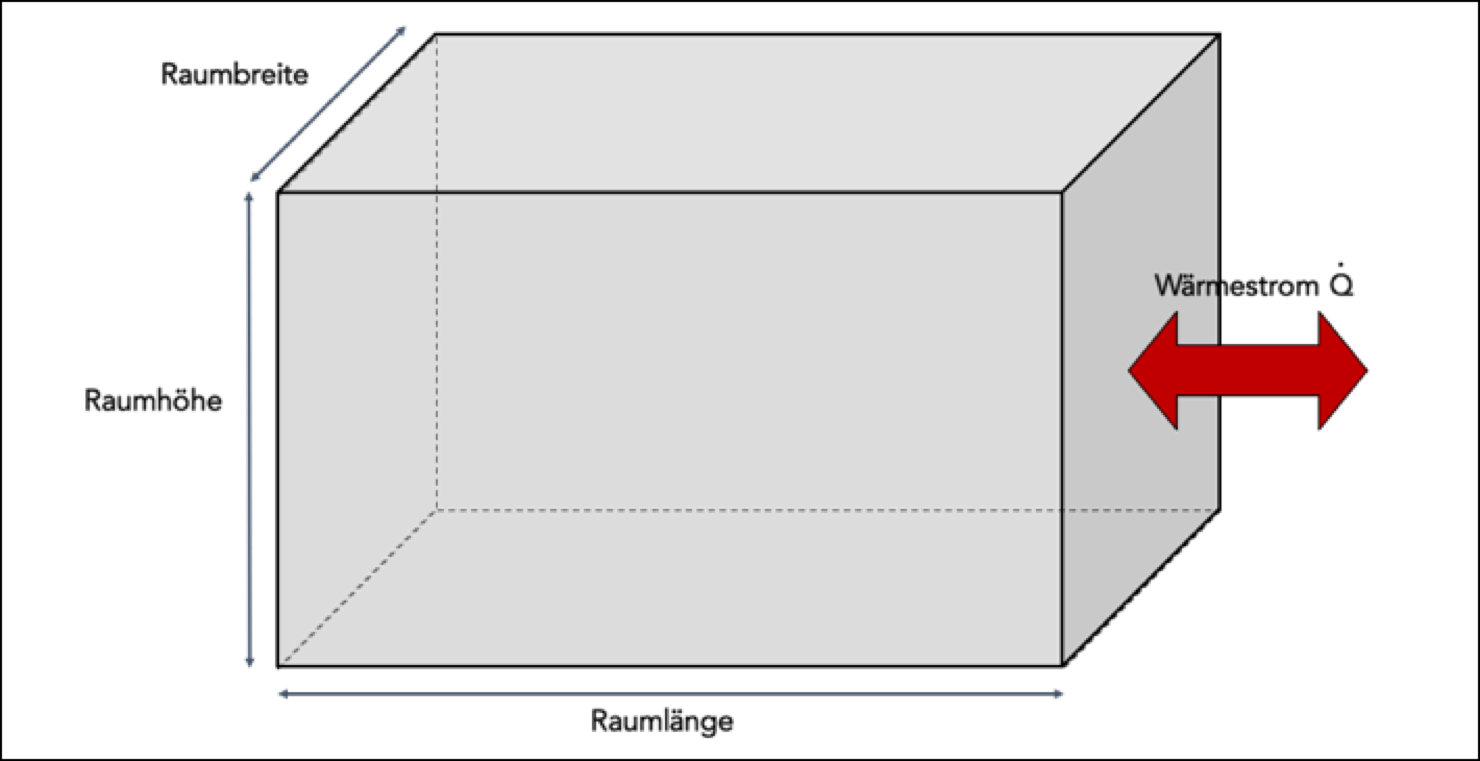
\includegraphics[width=\textwidth]{abbildungen/20160316_grundraum}
\caption{Grundmodell eines Raumes}
\label{fig:grundraum}
\end{figure}

Zur Bestimmung der Temperatur innerhalb des Raumes, ausgehend von einer initialen Raumtemperatur und dem externen Steuerungsparameter der Umgebungstemperatur, muss der Ausgleichsprozess zwischen Raum und Umgebung untersucht werden, konkret der ausgetauschte Wärmestrom. Um diesen nach \ref{eq:qdot} zu berechnen, müssen zunächst die verschiedene modellrelevante Eigenschaften des Raumes durch physikalische Größen und Variablen beschrieben werden. Zur Berechnung der Austauschoberfläche wird die Raumbreite, -länge und -höhe benötigt und weiterhin sind der U-Wert einer Betonwand, die spezifische Wärmekapazität und Dichte von Luft für die Bestimmung des Wärmestroms relevant.
Diese modellrelevanten Eigenschaften sind allesamt mit ihren Zahlenwerten in Tabelle \ref{tab:eigenschaften_raum} zusammengefasst.

\begin{table}[H]
\centering
\small
\renewcommand{\arraystretch}{1.3}
\begin{threeparttable}
\begin{tabularx}{1\textwidth}{p{0.5\textwidth}m{0.2\textwidth}m{0.18\textwidth}}
\toprule
\textbf{Modellrelevante Eigenschaften} & \textbf{Wert} & \textbf{Einheit} \\
\cmidrule[0.5pt](r{0.25em}){1-1} 
\cmidrule[0.5pt](l{0.25em}){2-2}
\cmidrule[0.5pt](l{0.25em}){3-3}

Raumbreite & 7,81\tnote{1)} & $[m]$ \\ 
\ccol Raumlänge & \ccol 5,78\tnote{1)} & \ccol $[m]$ \\
Raumhöhe & 2,99\tnote{1)} & $[m]$ \\
\ccol Wärmedurchgangskoeffizient Betonwand & \ccol 1,0\tnote{2)} & \ccol $[\frac{W}{m^{2}*K}]$\\
Spezifische Wärmekapazität von Luft & 1.000,0\tnote{3)} & $[\frac{J}{kg*K}]$\\
\ccol Dichte von Luft & \ccol 1,25 \tnote{3)} & \ccol $[\frac{kg}{m^{3}}]$\\
\bottomrule
\end{tabularx}
\begin{tablenotes}[]\footnotesize\singlespacing\setlength\labelsep{0pt}
\item[1)] Werte durch eigene Vermessung des Raumes K004b vom 07.12.2015.
\item[2)] Schätzwert, geschätzt nach \cite[S.~409]{re14} mit Richtwerten aus \cite[S.~194ff.]{re14}.
\item[3)] Tabellenwert aus \cite[S.~68]{ha13}.
\end{tablenotes}
\end{threeparttable}
\caption{Eigenschaften des Raummodells}
\label{tab:eigenschaften_raum}
\end{table}

Erfolgt nun die Bilanzierung des Raumes mit Hilfe des ersten Hauptsatzes der Thermodynamik nach \ref{eq:hauptsatz} und die Berechnung der inneren Energie des Raumes nach \ref{eq:innereenergie} ergibt sich folgendes, einfaches Gleichungssystem zur Bestimmung der Raumtemperatur in Abhängigkeit vom Steuergrößen Außentemperatur im Grundmodell in Modelica:

\begin{lstlisting}[language=Modelica,caption={Einfaches Gleichungssystem für das Grundmodell des Raumes in Modelica}, label=lst:grundraum]
equation
   /* calculate room volume */
   room_volume = room_length * room_height * room_breadth;
   /* calculate room mass */
   room_mass = room_volume * rho_air;
   /* calculate surface of heat exchange */
   exchange_surface = 2 * (room_length * room_breadth) + 2 * (room_length * room_height) + 2 * (room_breadth * room_height);
   /* calculate inner energy*/
   room_u = room_mass * cp_air * room_temperature;
   /* calculate derivative of the inner energy */
   der(room_u) = environment_qdot;
   /* calculate heatflow between room and environment */
   environment_qdot = u_wall * exchange_surface * (environment_temperature - room_temperature);
\end{lstlisting}

Damit ist ein Grundmodell für einen Raum gebildet, wie in \ref{fig:grundraum} graphisch dargestellt, um die Temperatur innerhalb eines Raumes zu berechnen. Dieses wird im Folgenden nun schrittweise erweitert und zum Abschluss überprüft, ob es der Realität genüge zu trägt.


\subsection{Modellerweiterung durch Berücksichtigung der realen Umgebung}

Im nächsten Schritt wird das einfache Raummodell zunächst an die reale Umgebung des Raums K004b angepasst. Die Lage von K004b ist in \ref{fig:skizzek004a} ersichtlich und es ist zu erkennen, dass der Raum lediglich zwei Außenwände besitzt, die an die Umgebungsluft grenzen: Die Wände in Richtung Süden und Westen. Die anderen beiden Wände, sowie die Decke und der Boden, grenzen an weitere Gebäudeteile des K~Gebäudes. Somit entspricht der Raum im Modell nach wie vor einem geschlossenen System und bildet weiterhin, zusammen mit dem umgebenden K~Gebäude und der Umgebungsluft, ein abgeschlossenes System. Jedoch müssen nun potenziell verschiedene Wärmeströme zwischen dem Raum und der Außenumgebung sowie dem Raum und dem K~Gebäude betrachtet werden. Da die fließenden Wärmeströme im Vergleich zur sehr großen Energie innerhalb des gesamten K~Gebäudes und der Umgebung nur verschwindend gering sind, wird der erwärmende beziehungsweise kühlende Effekt der Wärmeströme auf die beiden Teilsysteme vernachlässigt und es wird von konstanten, homogenen Temperaturen beider ausgegangen.

Durch diese Erweiterung des Modells hängt die Raumtemperatur nun von zwei Wärmeströmen und damit indirekt von zwei externen Steuergrößen, den Temperaturen in der Umgebung und im K~Gebäude, ab. Um die Wärmeströme separat berechnen zu können, wird die gesamte Oberfläche zum Wärmeaustausch aufgeteilt in die Austauschoberfläche mit der Umgebung und die Austauschoberfläche mit dem K~Gebäude. Des Weiteren werden im Modell die Temperatur der Außenumgebung und die Temperatur innerhalb des K~Gebäudes als externe Steuergrößen berücksichtigt. Das Gleichungssystem des Grundmodells in \ref{lst:grundraum} erweitert sich also um folgende Änderungen:

\begin{lstlisting}[language=Modelica, caption={Erweitertes Gleichungssystem Modell des Raumes unter Berücksichtigung der realen Umgebung in Modelica}, label=lst:raumeins]
equation
   [...]
   /* calculate surface of heat exchange with the environment */
   environment_surface = room_length * room_height + room_breadth * room_height;
   /* calculate surface of heat exchange with the remaining building */
   building_surface = 2 * (room_length * room_breadth) + room_length * room_height + room_breadth * room_height;
   /* calculate derivative of the inner energy */
   der(room_u) = environment_qdot + building_qdot;
   /* calculate heatflow between room and environment */
   environment_qdot = u_wall * environment_surface * (environment_temperature - room_temperature);
   /* calculate heatflow between room and building */
   building_qdot = u_wall * building_surface * (building_temperature - room_temperature);
\end{lstlisting}

Damit wurde das Raummodell an die reale Umgebung angepasst und um die Temperatur innerhalb des Raumes zu bestimmen, wird nun neben der Ausgangstemperatur im Raum und der Umgebungstemperatur noch die Temperatur innerhalb des restlichen K~Gebäudes berücksichtigt. Im nächsten Schritt werden die realen, räumlichen Gegebenheiten im Modell abgebildet.


\subsection{Modellerweiterung durch Berücksichtigung der räumlichen Gegebenheiten}

Um das Modell an die realen Gegebenheiten des Raumes K004b anzupassen, müssen zwei bauliche Gegebenheiten beachtet werden. Wie in \ref{fig:skizzek004a} bereits dargestellt ist, ist in der südlichen Außenwand eine Fensterfront vorhanden. Da der U-Wert eines Fensters erheblich von dem U-Wert einer Wand abweicht, entsteht ein zusätzlicher Wärmestrom zwischen dem Raum und der Umgebung durch das Fenster hindurch. Das Öffnen und Schließen der Fenster mit daraus resultieren Massenströmen wird zunächst nicht explizit berücksichtigt, weshalb das Raummodell weiterhin als geschlossenes System betrachtet wird. Des Weiteren ist es möglich, den Raum über einen Heizkörper zu beheizen. Mit dem Heizkörper, der zunächst als einfache Wärmequelle im Modell ergänzt wird, erhöht sich die Anzahl der externen Steuergrößen erneut, da die Temperatur innerhalb des Raumes auch von dieser abhängig ist.

Durch diese Erweiterungen werden auch weitere physikalische Größen zur Beschreibung der Eigenschaften des Raummodells benötigt. Wie bereits erwähnt werden die Eigenschaften um den U-Wert eines Fensters, sowie die Breite und Höhe der Fensterfront ergänzt, wie in Tabelle \ref{tab:eigenschaften_raumerw} zusammengefasst.

\begin{table}[H]
\centering
\small
\renewcommand{\arraystretch}{1.3}
\begin{threeparttable}
\begin{tabularx}{1\textwidth}{p{0.5\textwidth}m{0.2\textwidth}m{0.18\textwidth}}
\toprule
\textbf{Modellrelevante Eigenschaften} & \textbf{Wert} & \textbf{Einheit} \\
\cmidrule[0.5pt](r{0.25em}){1-1} 
\cmidrule[0.5pt](l{0.25em}){2-2}
\cmidrule[0.5pt](l{0.25em}){3-3}

Fensterbreite & 7,0\tnote{1)} & $[m]$ \\ 
\ccol Fensterhöhe & \ccol 2,08\tnote{1)} & \ccol $[m]$ \\
Wärmedurchgangskoeffizient Glas & 2,0\tnote{2)} & $[\frac{W}{m^{2}*K}]$\\

\bottomrule
\end{tabularx}
\begin{tablenotes}[]\footnotesize\singlespacing\setlength\labelsep{0pt}
\item[1)] Werte durch eigene Vermessung des Raumes K004b vom 07.12.2015.
\item[2)] Tabellenwert, geschätzt nach \cite[S.~270ff.]{h2000}.
\end{tablenotes}
\end{threeparttable}
\caption{Weitere Eigenschaften des Raummodells}
\label{tab:eigenschaften_raumerw}
\end{table}
 
Durch diese Anpassung verändert sich die Austauschoberfläche mit der Umgebung, die sich nun auf zwei Flächen mit verschiedenen Wärmedurchgangskoeffizienten verteilt. Des Weiteren wird eine Wärmequelle für die Heizung ergänzt, so dass sich folgende Änderungen des Gleichungssystems im Vergleich zum bisherigen Modell in \ref{lst:grundraum} ergeben:

\begin{lstlisting}[language=Modelica, caption={Erweitertes Gleichungssystem des Raumes unter Berücksichtigung der räumlichen Gegebenheiten in Modelica},label=lst:raumzwei]
equation
   [...]
   /* calculate surface of heat exchange with the environment */
   environment_surface = room_length * room_height + room_breadth * room_height - window-surface;
   /* calculate surface of heat exchange with the remaining building */
   building_surface = 2 * (room_length * room_breadth) + room_length * room_height + room_breadth * room_height;
   /* calculate surface of window with the environment */
   window_surface=(window_length*window_height);
   /* calculate derivative of the inner energy */
   der(room_u) = environment_qdot + building_qdot + window_qdot + radiator_qdot;
   /* calculate heatflow between room and environment through the walls */
   environment_qdot = u_wall * environment_surface * (environment_temperature - room_temperature);
   /* calculate heatflow between room and environment through the window */
   building_qdot = u_glass * window_surface * (environment_temperature - room_temperature);
   /* calculate heatflow between room and building */
   building_qdot = u_wall * building_surface * (building_temperature - room_temperature);
\end{lstlisting}

Damit ist das Modell auch an die räumlichen Gegebenheiten angepasst und beschreibt dadurch die realen Zusammenhänge in groben Zügen. Die bisherigen Zusammenhänge des Modells sind in \ref{fig:raumeins} graphisch dargestellt. Allerdings kann ein Controller die Heizung nicht beliebig als einfache Wärmequelle einsetzen. Daher wird im folgenden Abschnitt ein detaillierteres Modell des Heizkörpers gebildet, um die Steuerung für den Controller zu ermöglichen. 

\begin{figure}
\centering
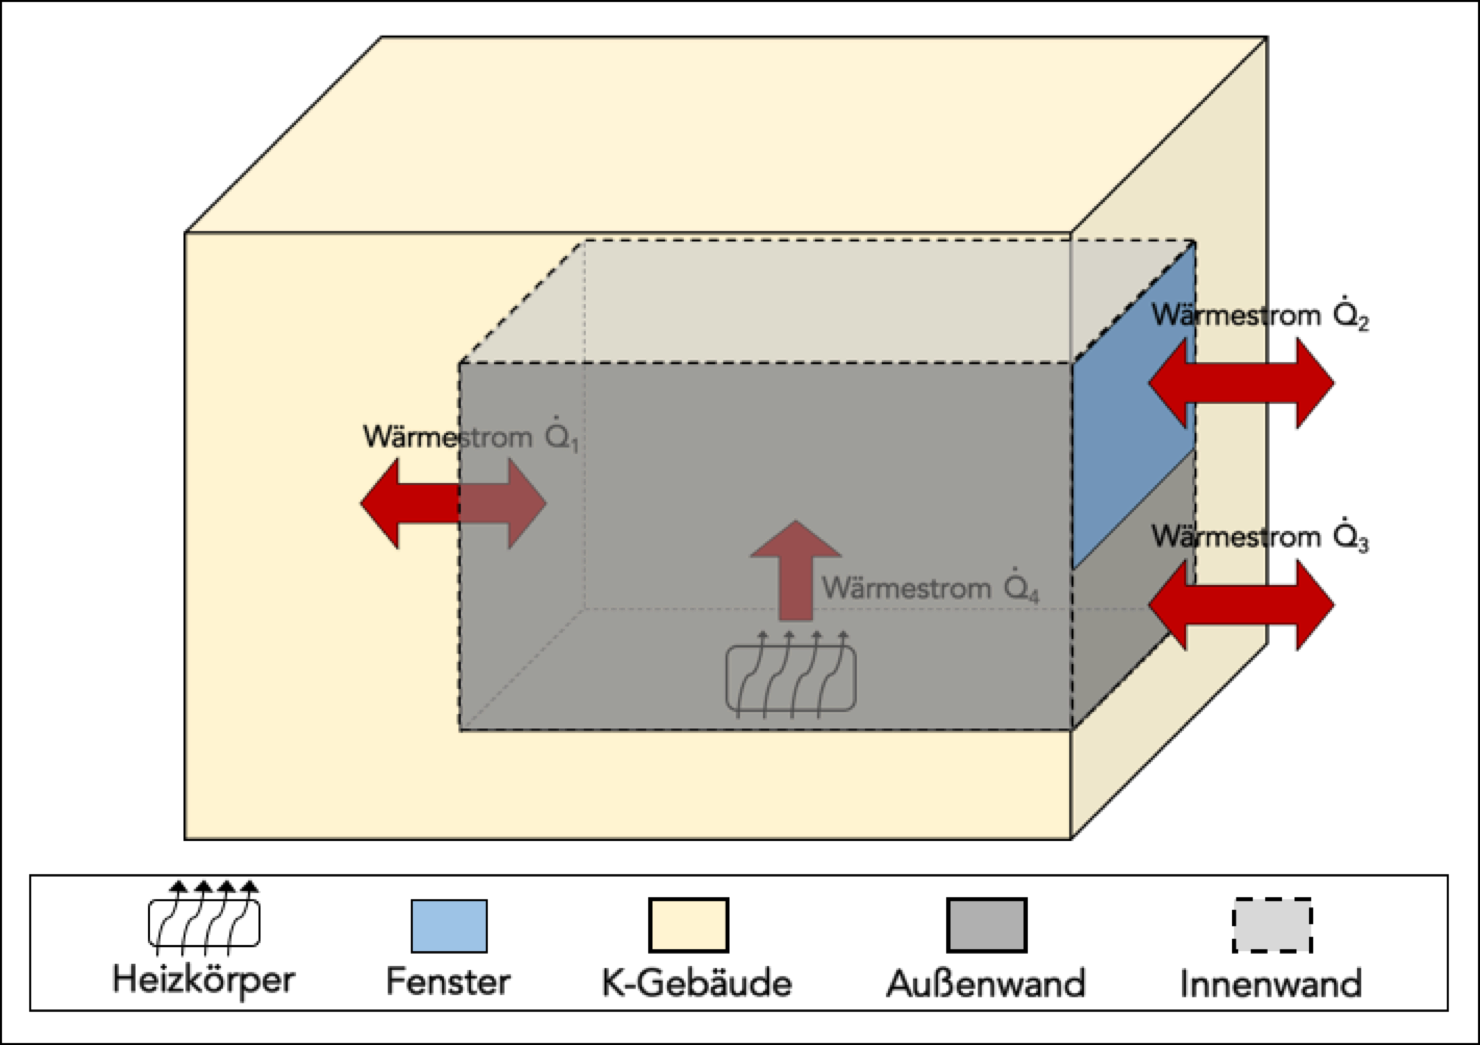
\includegraphics[width=\textwidth]{abbildungen/20160316_raumeins}
\caption{Erweitertes Raummodell}
\label{fig:raumeins}
\end{figure}



\subsection{Das Heizkörpermodell}

Der Heizkörper im Raum K004b lässt sich nach \cite[S.~824f.]{re14} als Stahlrohrradiator identifizieren. Er besteht aus genormten zwei-säuligen Gliedern, die jeweils am Sammler oben und unten miteinander verschweißt den Heizkörper bilden. Dabei sind die Temperatur des Heizwassers am Einlass des Heizkörpers und der Massenstrom wiederum Steuergrößen für das Modell. Die Temperatur am Einlass wird durch die Heizanlage vorgegeben und ist damit eine externe Steuergröße. Der Massenstrom wird direkt durch den Stellantrieb gesteuert und ist daher eine Steuergröße, die vom Controller mittelbar genutzt werden kann, um aktiv einen Einfluss auf die Raumtemperatur zu nehmen. Da der eingebrachte Wärmestrom nicht linear von der Temperaturdifferenz abhängt, erfolgt eine Diskretisierung des Heizkörpers in Volumenelemente, um den Heizkörper adäquat im Modell abzubilden. 

Zur Berechnung des in den Raum eingebrachten Wärmestroms, erfolgt wiederum eine Bilanzierung von jedem diskreten Volumenelement durch den ersten Hauptsatz der Thermodynamik nach \ref{eq:hauptsatz}. Der gesamte Wärmestrom berechnet sich dann aus der Summe der einzelnen Wärmestrome zwischen Raum und den Volumenelementen, welche sich nach \ref{eq:qdot} berechnen. Bei der Diskretisierung wird mit Hilfe der Heizwassertemperatur am Einlass des Volumenelements die Temperatur am Auslass berechnet und zusammen mit dem Massenstrom an das nächste Volumenelement weitergereicht.
Allerdings müssen für die Berechnung zunächst noch weitere Eigenschaften in das Raummodell mit aufgenommen werden, welche in \ref{tab:eigenschaften_heiz} zusammen mit ihren Werten dargestellt sind.

\begin{table}[H]
\centering
\small
\renewcommand{\arraystretch}{1.3}
\begin{threeparttable}
\begin{tabularx}{1\textwidth}{p{0.5\textwidth}m{0.2\textwidth}m{0.18\textwidth}}
\toprule
\textbf{Modellrelevante Eigenschaften} & \textbf{Wert} & \textbf{Einheit} \\
\cmidrule[0.5pt](r{0.25em}){1-1} 
\cmidrule[0.5pt](l{0.25em}){2-2}
\cmidrule[0.5pt](l{0.25em}){3-3}


Zahl der Glieder & 106\tnote{1)} & Stück \\ 
\ccol Säulen pro Glied & \ccol 2\tnote{1)} & \ccol Stück \\
Rohrdurchmesser Vertikal & 0,0255\tnote{1)} & $[m]$\\
\ccol Rohrdurchmesser Horizontal & 0,05 \ccol 2\tnote{1)} & \ccol $[m]$ \\
Höhe der Glieder & 0,4\tnote{1)} & $[m]$\\
\ccol Länge des Glieds & 0,045 \ccol 2\tnote{2)} & \ccol $[m]$ \\
Wassermasse innerhalb eines Gliedes & 0,35\tnote{2)} & $[kg]$\\
\ccol Spezifische Wärmekapazität von Wasser &\ccol 4.200,0\tnote{4)} &\ccol $[\frac{J}{kg*K}]$\\
Wärmedurchgangskoeffizient Heizkörper & 16\tnote{3)} & $[\frac{W}{m^{2}*K}]$\\
\ccol Anzahl Volumenelemente & \ccol 10&\ccol  Stück\\

\bottomrule
\end{tabularx}
\begin{tablenotes}[]\footnotesize\singlespacing\setlength\labelsep{0pt}
\item[1)] Wert aus eigener Vermessung des Raumes K004b vom 07.12.2015.
\item[2)] Tabellenwert, entnommen aus \cite[S.~825]{re14}.
\item[3)] Tabellenwert, geschätzt nach \cite[S.~191ff.]{re14}.
\item[4)] Tabellenwert, entnommen aus \cite[S.~619]{ba12}.
\end{tablenotes}
\end{threeparttable}
\caption{Eigenschaften des Heizkörpermodells}
\label{tab:eigenschaften_heiz}
\end{table}

Die realen Eigenschaften des Heizkörpers werden eins zu eins im Modell abgebildet und anschließend im Heizkörpermodell zentral auf die einzelnen diskretisierten Volumenelemente umgerechnet, wie in Listing \ref{lst:heiz} in Zeile  zu sehen. Dazu gehört die Zahl und Wassermasse der Glieder, die Höhe des Heizkörpers sowie die Anzahl, Durchmesser und Längen der verschiedenen Rohre, um die Wärmeaustauschoberfläche zu bestimmen. Zudem werden die spezifische Wärmekapazität des Heizwassers und der Wärmedurchgangskoeffizient des Heizkörpers benötigt.

\lstinputlisting[language=Modelica ,caption={Auszüge des Modelica Modells vom Heizkörper in K004b}, label=lst:heiz, linerange={20-20, 47-57,58-60, 106-120}]{listings/room_model_listing.mo}

Das Modell des Heizkörpers ist als Subkomponente in den Raum integriert und die Steuergrößen werden über einen eigenen Port am Raummodell an den Heizkörper übergeben. Mit dem Modell des Heizkörpers wird ein physikalisch motivierter, mittelbarer Zusammenhang zwischen der Heizleistung und dem Massenstrom hergestellt, welcher insbesondere von einem modellprädiktiv regelnden Controller genutzt werden kann.

Bereits bei den Einsatzzielen der Anlage in Abschnitt\ref{sec:anforderungen} war gefordert, den Zusammenhang zwischen der Sonneneinstrahlung und der Raumtemperatur zu untersuchen sowie Störgrößen explizit in Kauf zu nehmen. Daher ist es passend, dass die Fensterfront in Richtung Süden ausgerichtet ist und der Raum K004b als Büro genutzt wird. Um jedoch das Modell darauf anzupassen, erfolgt im nächsten Abschnitt erfolgt weitere Erweiterung des Modells.


\subsection{Modellerweiterung durch Berücksichtigung der Sonneneinstrahlung und Störgrößen}
\label{sub:modsonne}

Der Raum K004b wird regulär als Büro genutzt, weshalb verschiedene Faktoren als Störgrößen in Bezug auf die Raumtemperatur betrachtet werden können. Zum einen wird durch die Menschen und deren Rechner weitere Wärme in den Raum eingebracht und zum anderen werden die Fenster und die Türen geöffnet und geschlossen. Dabei werden Massenströme zwischen Raum und Außenumgebung sowie K~Gebäude ausgetauscht, welche jedoch zunächst nicht modelliert werden sollen, sondern als Störgröße betrachtet die es durch die Modellprädiktive Regelung zu auszugleichen gilt. Die Wärme von Rechnern und Menschen werden als einfache Wärmequelle im Modell berücksichtigt. 
Zudem trifft auf die südseitigen Fenster Sonnenstrahlung, welche ebenfalls einen Wärmestrom in den Raum einbringt und damit ebenfalls einen Einfluss auf die Raumtemperatur hat. Dieser wird zunächst ebenfalls als eine einfache Wärmequelle aufgefasst.
Damit ergeben sich zwei weitere äußere Steuergrößen, die von der Anlage beziehungsweise dem Modell nicht beeinflusst werden können. Damit erweitert sich das Modell wie folgt:

\begin{lstlisting}[language=Modelica, caption={Erweitertes Gleichungssystem Modell des Raumes unter Berücksichtigung der Sonneneinstrahlung und Störgrößen},label=lst:raumdrei]
equation
   [...]
   /* calculate derivative of the inner energy */
   der(room_u) = environment_qdot + building_qdot + window_qdot + radiator_qdot + sun_qdot + otherfactors_qdot;
\end{lstlisting}

\begin{figure}
\centering
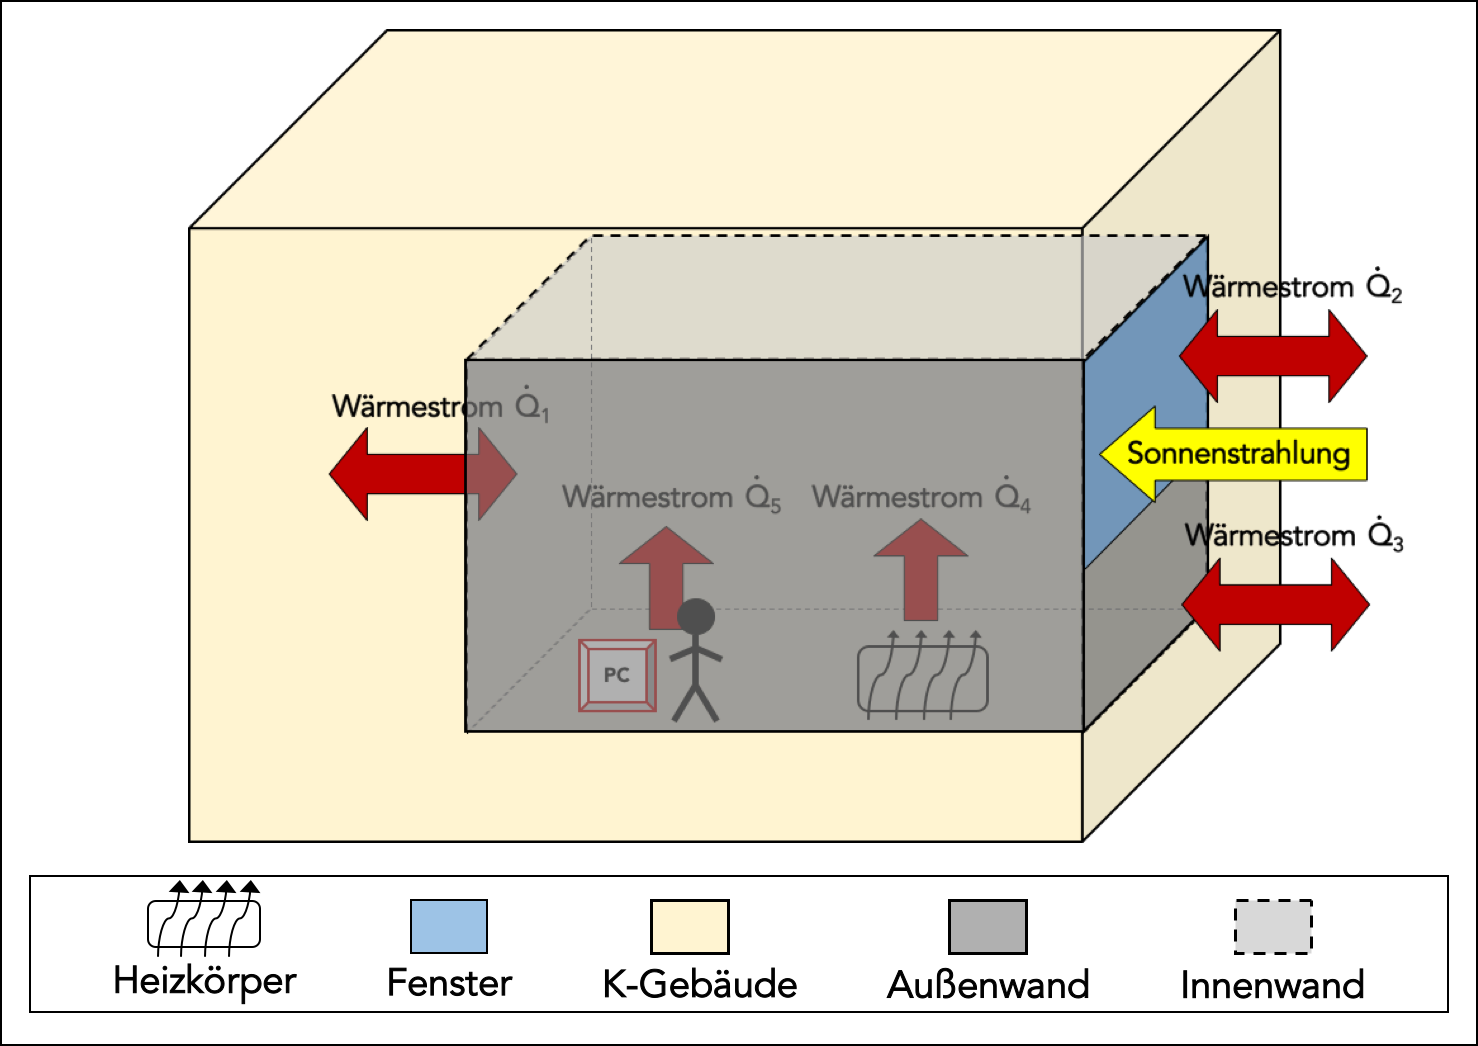
\includegraphics[width=\textwidth]{abbildungen/20160317_raumzwei}
\caption{Erweitertes Raummodell}
\label{fig:raumdrei}
\end{figure}


Damit lassen sich die Zusammenhänge des Modells wie in \ref{fig:raumdrei} visualisieren. Der Einfluss der Sonnenstrahlung wurde bereits in Kapitel \ref{sub:sonne} erläutert und muss nun an die Gegebenheiten des Raumes K004b angepasst werden. Als Messwerte stehen Werte der Globalstrahlung zur Verfügung, welche umgerechnet werden müssen in die effektive Strahlungsintensität an der Fenstersfront.

Da zur Berechnung der effektiven Strahlungsintensität neben der Globalstrahlung auch der Azitmuth und Höhenwinkel der Sonne bekannt sein muss, werden komplexe Berechnungen nötig. Da die Sonnenstrahlung eine Steuergröße darstellt und um die Komplexität des Modells zu schonen, werden die Effektivwerte der Sonnenstrahlung von einem Python Skript berechnet und anschließend dem Modell übergeben. Zudem hat dies den Vorteil, dass im pysolar Package bereits sehr exakte Algorithmen implementiert sind. 
Das Programm ist in Listing \ref{lst:sonne} dargestellt. 
Zur Berechnung des Azimuth- und Sonnenhöhenwinkels werden der Längen- und Breitengrad des K-Gebäudes sowie die Höhe über dem Meerespiegel benötigt. Um die effektive Solarstrahlung zu Bestimmen wird zusätzlich die Ausrichtung der Fensterfläche benötigt. Die Werte sind in Listing \ref{lst:sonne} in Zeile sieben bis zehn zu finden und wurden mit Hilfe von \cite{go15} ermittelt.

\lstinputlisting[language=Python ,caption={Programm zur Umrechnung der Globalstrahlung in die effektive Solarstrahlung an der Fensterfront am Rum K004b}, label=lst:sonne]{listings/radiation_conversion_k004b.py}

Außerdem wird der Startzeitpunkt und der Abstand zwischen den Messpunkten für die gemessenen Daten benötigt, da der Stand der Sonne von der Uhrzeit abhängig ist. Nach dem Einlesen der Messdaten aus der Datei globalstrahlung.csv wird anschließend für jeden einzelnen Messwert und -zeitpunkt der Azimuth- und Sonnenhöhenwinkel berechnet. Darauf basierend wird geprüft, ob die Sonne senkrecht am Himmel steht, noch nicht aufgegangen ist oder die Fläche verschattet ist. Ist dies der Fall trifft keine effektive Strahlung auf das Fenster. Des Weiteren würden sich für niedrige Sonnenstände sehr hohe und unrelistische effektive Strahlungswerte ergeben, weshalb diese für Sonnenstandswinkel kleiner als fünf Grad begrenzt werden.
Ansonsten wird der effektive Strahlungswert nach REFXXXXXgleichung berechnet und in der Datei qdotsun-effective gespeichert. Dieses Programm kann in leicht abgewandelter Form einfach zur Umrechnung einzelner Messwerte genutzt werden, indem das Einlesen und Speichern der umgerechneten Daten durch eine Abfrage eines Messwertes und Übergabe einer Variable mit umgerechnetem Messwert ersetzt wird.

Der effektive Strahlungswert wird allerdings durch den Transmissionsgrad des Fensters weiter abgeschwächt, der durch einen weiteren Paramater/ eine weitere Eigenschaft der $window\_transmission$ beschrieben wird. Der Schätzwert für eine zweischeibige Verglasung des Fensters stammt aus \cite[S.~63]{ha13}. Dadurch erweitert sich das Modell um ein Fenster als Subomponente:

\begin{lstlisting}[language=Modelica, caption={Fenster als Subkomponente des Raummodells},label=lst:raumdrei]
model Window
	Modelica.SIunits.DensityOfHeatFlowRate qdotsun_effective;
	Modelica.SIunits.HeatFlowRate qdot_effective;
	parameter Real window_transmission = 0.5;
	Modelica.SIunits.Area window_surface;
  equation
  	qdot_effective = qdotsun_effective * window_transmission * window_surface;
end Window;
\end{lstlisting}

Die Modellkomplexität ist bis zu diesem Punkt noch überschaubar und weiterhin berücksichtigt das Modell die physikalischen Effekte mit dem größten bzw. mit relevanten Einfluss. Damit ist die Modellbildung abgeschlossen und das gesamte Modell des Raumes findet sich im Anhang \ref{att:raummod}. Bei der Modellbildung wurde auf eine Programmierung mit klarer Struktur wert gelegt. Daher sind die Variablen der Modelle strikt nach Parametern, Controls und Zuständen gegliedert/sortiert.

 Das Schaltbild in Dymola, welches als Umgebung zur Modellbildung und Simulation genutzt wurde ist in REFXXXXX abgebildet. Darauf wird auch deutlich, dass das Modell 6 verschiedene Steuergrößen und damit Freiheitsgrade besitzt. Jedoch werden fünf davon durch äußere Bedingungen festgelegt, durch die Außentemperatur, die Temperatur im K~Gebäude, die Temperatur am Einlass der Heizung, die anderen Faktoren sowie die Solarstrahlung. Damit kann der Controller lediglich den Massenstrom zur Beeinflussung der Raumtemperatur nutzen um auf Änderungen der anderen Steuergrößen zu reagieren. 

FIG MOPDELICA

Weitere Effekte die explizit nicht berücksichtigt wurden sind die Energie innerhalb der Wände und des Mobiliars von Raum K004b, welche bei abrupter Abkühlung der Raumlufttemperatur einen stark erwärmenden Einfluss durch die Abstrahlung von Wärme, also Wärmekonvektion wie in Kapitel \ref{chap:theoretischegrundlagen} beschrieben. Da sich eine solch starke Abkühlung der Raumluft jedoch über einen längeren Zeithorizont erstreckt, wird diese als Störgröße wahrgenommen die ein Modellprädiktiver Regler ausgleichen können sollte.


\section{Simulation und Modellanpassung}

In diesem Abschnitt erfolgt zunächst die Simulation der Raumtemperatur unter Verwendung des Modells. Dazu werden für die Steuergrößen reale Messwerte vorgegeben, um die Güte des Modells abzuschätzen zu können, durch einen Vergleich der berechneten und tatsächlichen gemessen Werte. Abschließend erfolgt eine Anpassung der Modellparameter mit Hilfe von \cite{casiopeia}, um die Modellgüte zu verbessern.

\subsection{Simulation und Validierung des Modells}

Die Validation des Modells wird in zwei Schritte aufgeteilt. Zunächst wird das Raummodell ohne Verwendung des Heizkörpers simuliert, um das Grundmodell des Raumes zu überprüfen und ein Gefühl dafür zu bekommen ob alle wichtigen physikialischen Effekte berücksichtigt wurden. Im nächsten Schritt wird erfolgt eine Simulation, bei der der Heizkörper zum Einsatz kommt, die dazu dienen soll die Güte der Abbildung des Heizkörpers zu bestimmen.
Somit gilt es für den ersten Schritt Zeitintervall zu identifizieren, welches möglichst langer Dauer ist und währenddessen möglichst wenig Störfaktoren aufgetreten sind und weiterhin der Heizkörper nicht genutzt wurde. Ein solches Zeitintervall findet sich über die Weihnachten vom 23.12.2105 bis zum 28.12.2015, da aufgrund der Feiertage das Büro nicht genutzt wurde.
Das Intervall umfasst mehr als 5 Tage, von denen an den ersten Tage eine sehr milde Außentemperatur zwischen $8^{\circ}C$ und $16^{\circ}C$ vorgeherrscht hat. Erst am letzten Tag nähert sich die Außenlufttemperatur dem Gefrierpunkt von $0^{\circ}C$. Außerdem hat die Sonne gegen mittag geschienen und den Raum dadurch erwärmt.
Die genauen Messdaten in 10 minütigen Intervallen der Globalstrahlung und Außentemperatur für diesen Zeitraum wurden von \cite{wetter} zur Verfügung gestellt und sind in REFXXXXBILD visualisiert sowie auf der angehängten CD in der Datei XXXXXX zu finden.
Der Simulation wurde außerdem eine Temperatur von $22^{\circ}C$ im K~Gebäude und die gemessene Initialtemperatur von $22,8^{\circ}C$ zugrunde gelegt. Die Ergebnisse der Simulation sind im Plot in Abbildung \ref{fig:valid1} abgebildet und werden im Folgenden analysiert.

\begin{figure}
\centering
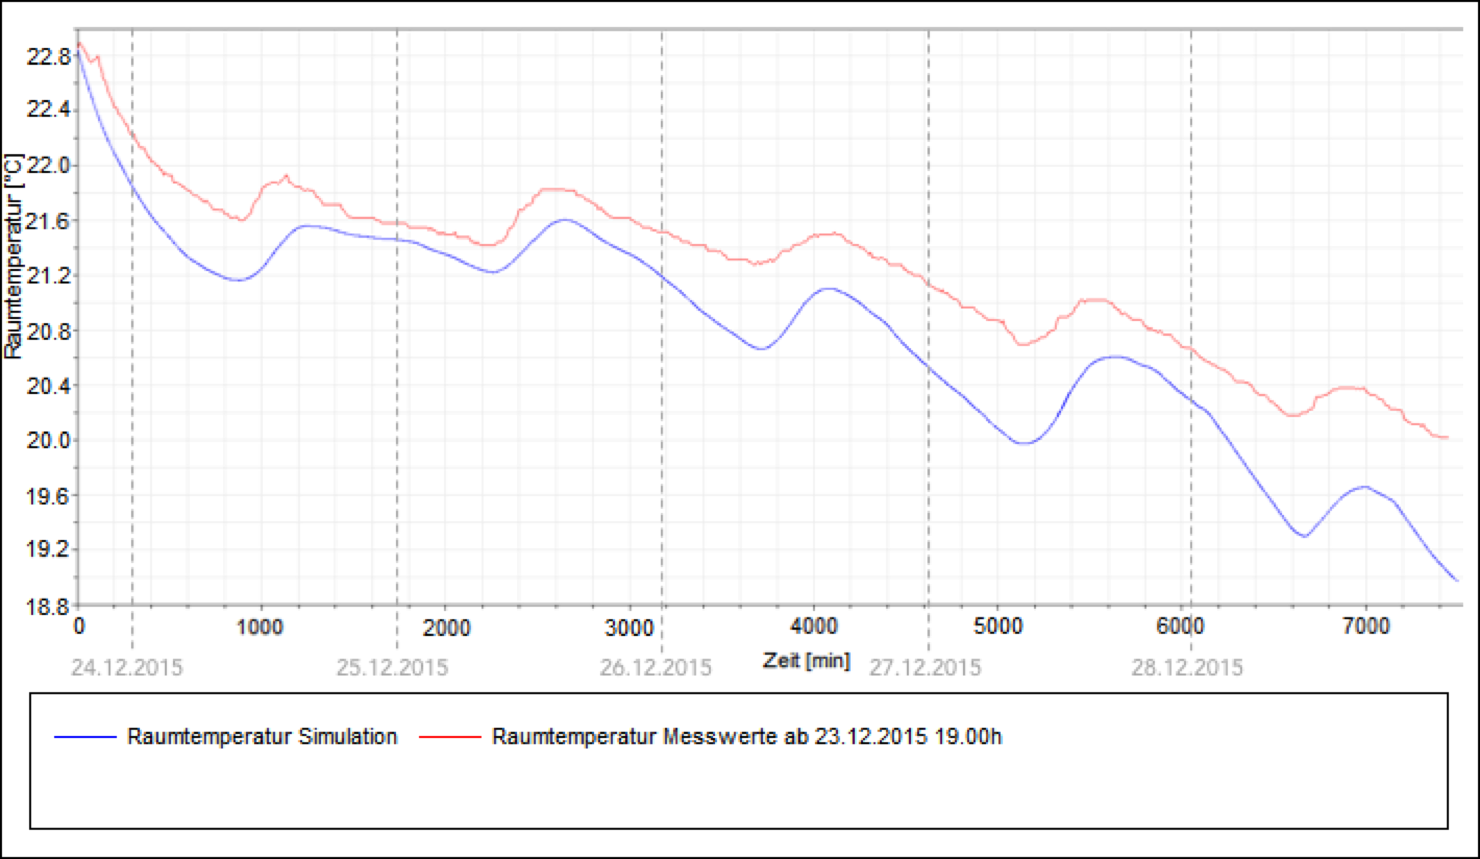
\includegraphics[width=\textwidth]{abbildungen/20160328_validierung1}
\caption{Simulation des Raummodells ohne Einsatz der Heizung}
\label{fig:valid1}
\end{figure}

Zu beachten ist die Skalierung der Abzisse, welche in Minutenschritte eingeteilt ist und die Simulation erstreckt über einen Zeitraum von 7500 Minuten. Im Rahmen der Modellprädiktiven Regelung werden die Simulationszeiträume deutlich kürzer betrachtet, jedoch soll durch diese Simulation ein Abgleich des Modells mit der Realität ermöglicht werden, worin sich die lange Periode begründet.

Der erste Blick lässt bereits erkennen, dass die simulierte Temperaturkurve eine ähnliche Dynamik wie der gemessene Temperaturverlauf aufweist. Von Beginn der Simulation bis hin zum 26.02.2016 stimmt das Systemverhalten sehr gut mit der Realität überein. Danach erfolgt ein leichter Knick bei der simulierten Kurve, der bis Ende der Simulation erhalten bleibt und nicht weiter erklärt werden kann. 
Außerdem ist eine minimale zeitliche Verzögerung des Modells zur Realität erkennbar, was auf einen Unterschied in der Trägheit zwischen Realität und Modell hindeutet.
Die simulierte Temperaturkurve liegt während des gesamten Intervalls unterhalb der Messwerte, was einen Hinweis auf einen zu hohen Wärmeverlust im Modell liefert.  
Des Weiteren lässt sich der Einfluss der Solarstrahlung auf die Raumtemperatur deutlich erkennen, der täglich etwa zur Mittagszeit einsetzt und den Raum dadurch bis Nachmittags erwärmt.

Insgesamt ist zu hervorheben, dass die simulierte von der tatsächlich gemessenen Temperatur innerhalb der ersten beiden Tag um nicht mehr als $0,4^{\circ}C$ und während der gesamten Simulationsdauer um nicht mehr als $1^{\circ}C$ abweicht.
Dabei besitzen die Temperatursensoren des \textsc{Webthermograph8x} eine Messabweichung von $\pm 0,26^{\circ}C$ und die beiden RTM1 Temperaturfühler eine Messabweichung von $\pm 0,5^{\circ}C$.
Außerdem haben die Messwerte der Wetterstation auf dem Physikhochhaus des Karlsruher Instituts für Technologie eine 10-minütige Auflösung, wohingegen die Raumtemperatur minütlich gemessen wurde.
Durch die örtliche Trennung von 1km Luftlinie zwischen der Messstation und dem K~Gebäude, ist es durchaus in Betracht zu ziehen, dass Messwerte durch eine Bewölkung die Steuergröße Solarstrahlung am Raum nicht vollständig, also mit fehlern behaftet beschreibt.

Im Rahmen der Modellprädikitiven Regelung werden jedoch wie zuvor erwähnt kürzere Simulationszeiträume im unteren Stunden beziehungsweise höheren Minutenbereich betrachtet, weshalb die Güte des Modells ohne Einsatz des Heizkörpers dazu ausreichend ist.

Im nächsten Schritt findet eine Simulation mit Einsatz des Heizkörpers statt, um das vollständige Modell mit der Realität abzugleichen. Der Heizkörper wurde für die folgende Modellsimulation in vier Volumenelemente diskretisisert.
Für diese Simulation wurde ein Zeitintervall gesucht, indem die Raumtemperatur unter die untere Schalttemperatur von $20^{\circ}C$ fällt, damit der Controller den Heizkörper zum Erwärmen des Raumes bis zum oberen Schaltpunkt von $21,5^{\circ}C$ nutzt und der Raum nach schließen des Heizkörperventils wieder abkühlt. Ein passendes Intervall findet sich vom 28.12.2015 bis zum 30.12.2015, dass auch an diesen Tagen das Büro nicht genutzt wurde.
Die Messdaten für die Globalstrahlung und Außenlufttemperatur wurden auch hier in 10 minütigen Intervallen von \cite{wetter} zur Verfügung gestellt und sind auf der angehängten CD in der Datei XXX zu finden. Die Sonne hat gegen Nachmittag des 29.12.2016 leicht geschienen und die Außenlufttemperatur hat sich zwischen 6 Grad leicht unter den Gefrierpunkt bewegt. Die Heizkörper wird gegen Nachmittag des 29.12.2015 bis bis gegen Abend genutzt.
Auch bei dieser Simulation wurde eine Temperatur von $22^{\circ}C$ im K~Gebäude und die gemessene Initialtemperatur von $21,25^{\circ}C$ zugrunde gelegt. Die Simulationsergebnisse sind im Plot \ref{fig:valid2} abgebildet und werden wiederum im Folgenden analysiert.

\begin{figure}
\centering
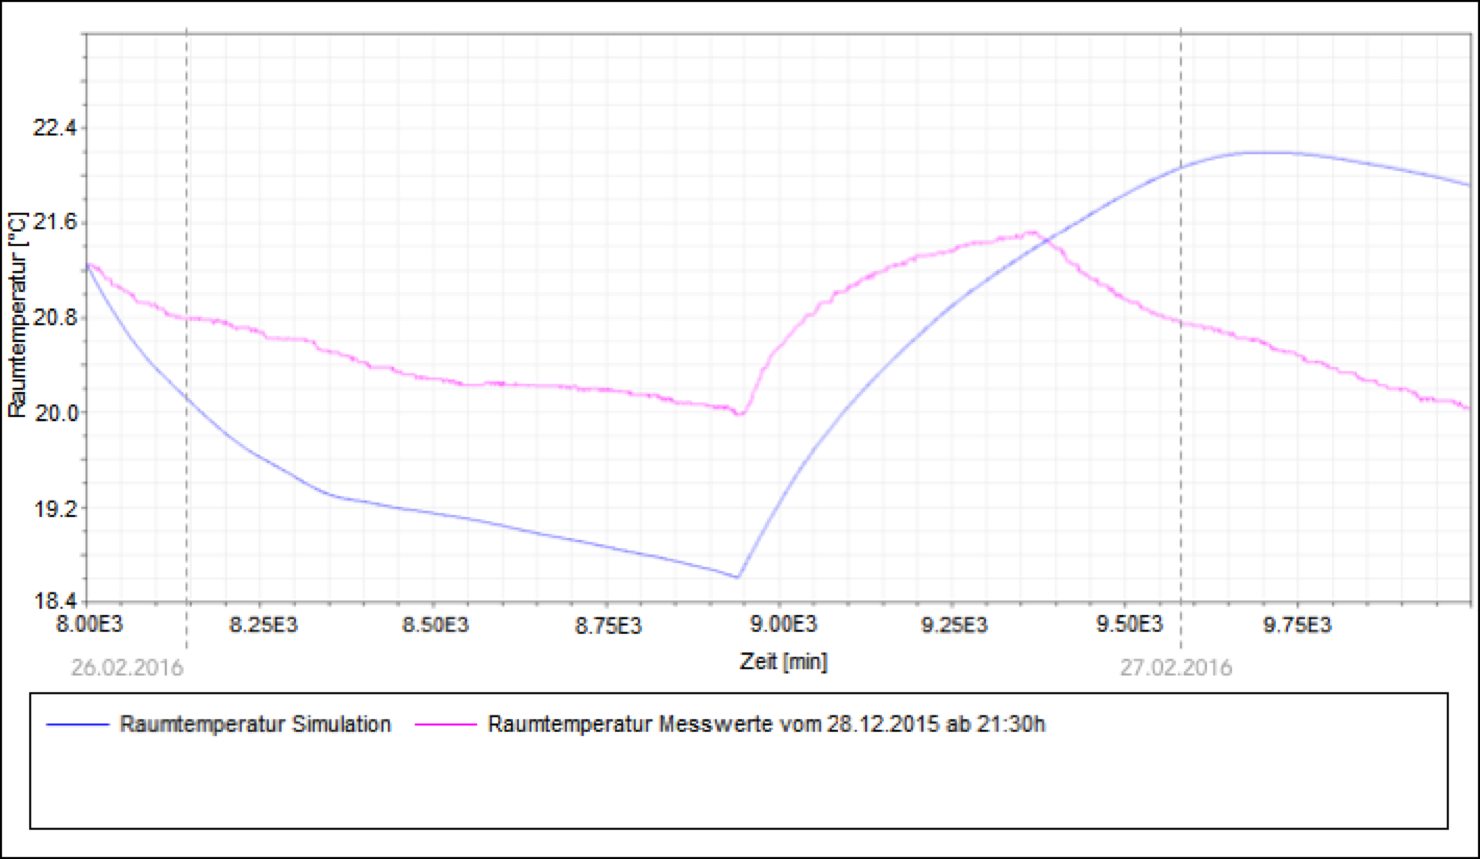
\includegraphics[width=\textwidth]{abbildungen/20160328_validierung2}
\caption{Simulation des Raummodells mit Einsatz des Heizkörpers}
\label{fig:valid2}
\end{figure}

Der Simulationszeitraum beginnt gegen späten Abend am 28.02.2015 und erstreckt sich über 2000 Minuten bis zum frühen Morgen des 30.12.2015. Die Simulationsergebnisse bestätigen zunächst die vorherigen Ergebnisse, indem das Modell zunächst schneller auskühlt als der reale Raum. Dies liefert wiederum einen Hinweis auf einen zu hohen Wärmeverlust im Modell.
Die Systemdynamik des Modells folgt in etwa der Realität bis zur Nutzung des Heizkörpers nach etwa 950 simulierten Minuten. 
Das Öffnen des Heizkörperventils ist sowohl im Modell, als auch in den Messwerten sehr gut zu sehen und führt zu einem signifikanten Anstieg der Raumtemperatur. Es wird zudem deutlich, dass die Modellreaktion zum einen gleichzeitig einsetzt, jedoch deutlich langsamer/träger abläuft als in der Realität. Zum anderen wird im Modell weitaus mehr Wärme in den Raum eingebracht als in der Realität, was auf eine erhöhte Wärmezufuhr durch den Heizkörper oder durch die Solarstrahlung hinweist, da wie zuvor erwähnt die lokale Bewölkung für Fehler sorgen könnte.
Die Trägheit des Modells kann auf eine unzureichende Diskretisierung hinweisen, weshalb die Anzahl der Volumenelemente auf 10 erhöht wurde. Die anschließenden Untersuchungen zeigen, dass die Modellgüte damit gesteigert werden konnte.

Insbesondere im Zusammenhang mit den zuvor festgestellten Unsicherheiten bei den Messwerten lässt sich feststellen, dass die  Simulationskurve die Dynamik des realen Systems erkennbar widerspiegelt, wenn auch mit einer gewissen Trägheit verbunden durch die Nutzung der Heizung.

Zusammenfassend lässt sich feststellen, dass das Modell die grundlegende Systemdynamik der Realität beschreibt, jedoch noch gewisse Abweichungen im Modell vorhanden sind. Dies wurde insbesondere durch die sehr langen Simulationsintervalle deutlich, die für den späteren Einsatz des Modells nicht von weiterer Relevanz sind.

 Um die Modellgüte insbesondere hinsichtlich des Einsatzes der Heizung zu verbessern, wird im Folgenden eine Parameterschätzung vorgenommen und abschließend überprüft, ob das Modell den Anforderungen für eine Modellprädiktive Regelung mit \textsc{JModelica.org} genügt.


\subsection{Anpassung des Modells}
Ziel des Abschnittes ist eine Verbesserung des Raummodells, welche durch eine Parameterschätzung mit \cite{casiopeia}, einer freien Softwareumgebung für die optimale Versuchsplanung und Parameterschätzung.
Wie bereits erwähnt, werden beim Einsatz des Modells mit Modellprädiktiver Regelung kürzere Intervalle betrachtet, weshalb die Modelloptimierung anhand von kürzeren Intervallen erfolgt. Die Durchführung der Parameterschätzung erfolgte mit freundlicher Unterstützung von Herrn \textsc{Adrian Bürger}, der das Übersetzen des Modell und die Ausführung übernommen hat.

Wie bereits zuvor, erfolgt auch die Parameterschätzung systematisch, um die einzelnen Modellparameter anzupassen. Als zu schätzende Parameter wird der Wärmedurchgangskoeffizient der Raumwände und des Heizkörpers sowie der Transmissionsgrad der Fensterscheiben betrachtet, welche im Folgenden in drei Schritten berechnet werden. Der Wärmedurchgangskoeffizient der Glasscheibe wird als fester Wert angenommen, da sich aufgrund der offensichtlichen Korrelation zwischen den beiden Wärmedurchgangskoeffizienten voneinander nicht-physikalische Schätzwerte ergeben können.

Es muss weiterhin beachtet werden, dass die Erhöhung der Modellgüte durch den Einsatz realer Messwerte ebenfalls mit einer Abweichung der physikalischen Schätzparameter zur Realität einhergehen können, da Störgrößen und Messfehler implizit berücksichtigt werden.

Zunächst wird der Wärmedurchgangskoeffizient der Wand bestimmt, wozu Intervalle genutzt wurden die möglichst ohne Störgrößen sind und ohne Einsatz der Heizung auskommen. Dazu bieten sich Zeitintervalle am Abend an, an denen das Büro nicht mehr genutzt wird und keine Solarstrahlung mehr auf die Fenster trifft. Das Ergebnis der Parameterschätzung für zwei Intervalle ist in den Plots in \ref{fig:step1} dargestellt. Das Skript zur Parameterschätzung findet sich im Anhang \ref{att:cd} in der Datei $room_pe_step1_night.py$.

\begin{figure}
\centering
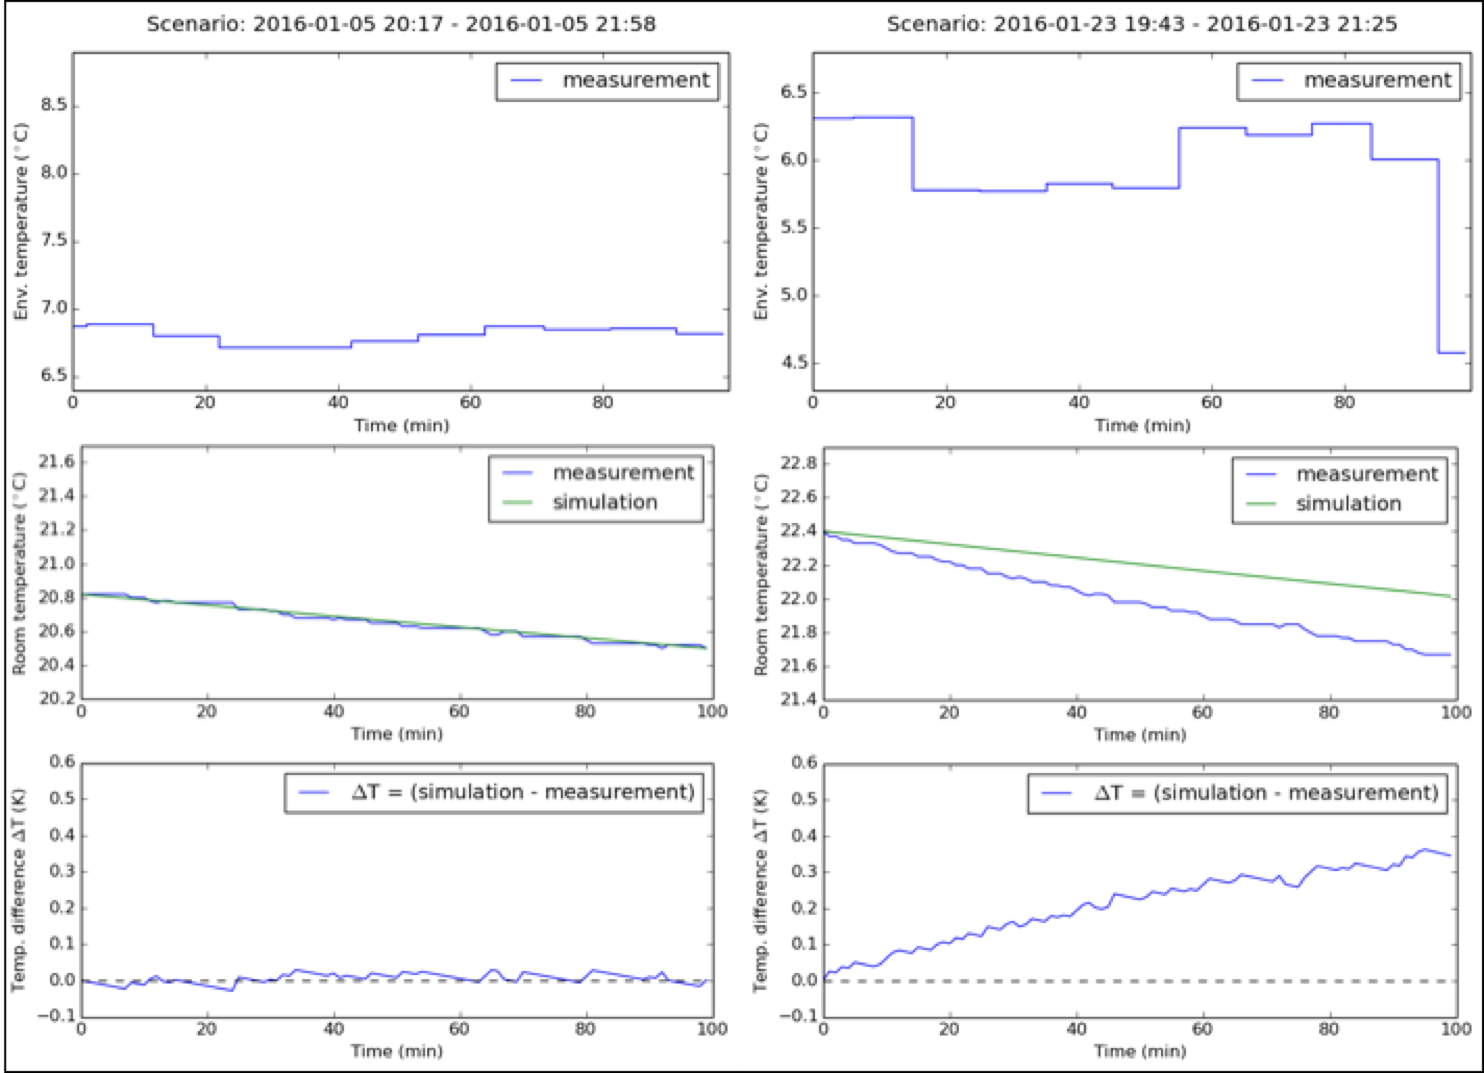
\includegraphics[width=\textwidth]{abbildungen/20160329_pestep1}
\caption{Parameterschätzung des Wärmedurchgangskoeffizienten der Wand von zwei Intervallen}
\label{fig:step1}
\end{figure}

Die Plots auf der linken Seite stellen das Ergebnis für ein 100-minütiges Intervall vom Abend des 05.01.2016, auf der rechten Seite vom Abend des 23.01.2016 dar. Mit dem vorab fixierten U-Wert für Glas ergab sich ein Schätzwert für den Wärmedurchgangskoeffizient der Wand von $U_{wall}=0.612986$ .

Die oberen beiden Plots enthalten die Verläufe der Steuergröße Außenlufttemperatur im Intervall, wobei die Solarstrahlung und die Heizung keinen Einfluss hatten. Die genauen Messdaten sind den Dateien auf der angehängten CD in \ref{att:cd} im Ordner enthalten. Die mittleren Plots zeigen einen Vergleich der gemessen Raumtemperatur mit der Simulation des geschätzten Intervalls über 100 Minuten. Darin ist gut zu erkennen, dass die Dynamik des Modells durch eine Anpassung des Parameters weiter verbessert werden konnte. Die unteren Plots zeigen die Abweichung zwischen Simulation und Messwerten. Im linken Intervall beschreibt die Simulation bis auf minimale Abweichungen das reale System sehr genau, im Rechten ergibt sich bei der Simulation ein leicht erhöhte Temperatur im Vergleich zur Messung, die mit einer Abweichung von etwa $0,35^{\circ}C$ nach 100 Minuten immer noch eine ausreichende Güte besitzt.

Im nächsten Schritt wird der Transmissionsgrad der Fensterscheiben geschätzt. Dazu wurden wiederum Intervalle identifiziert, an denen die Sonne geschienen hat und die Störgrößen und den Einsatz der Heizung möglichst ausschließen. Dazu bieten sich zwei Intervalle Anfang Januar an, am 02.01.2016 und 05.01.2016 gegen die Mittagszeit, an denen das Büro nur teilweise genutzt wurde. Die Ergebnisse der Schätzung sind in \ref{fig:step2} zusammengefasst. Das Skript zur Parameterschätzung findet sich im Anhang \ref{att:cd} in der Datei $room_pe_step2_day.py$.

\begin{figure}
\centering
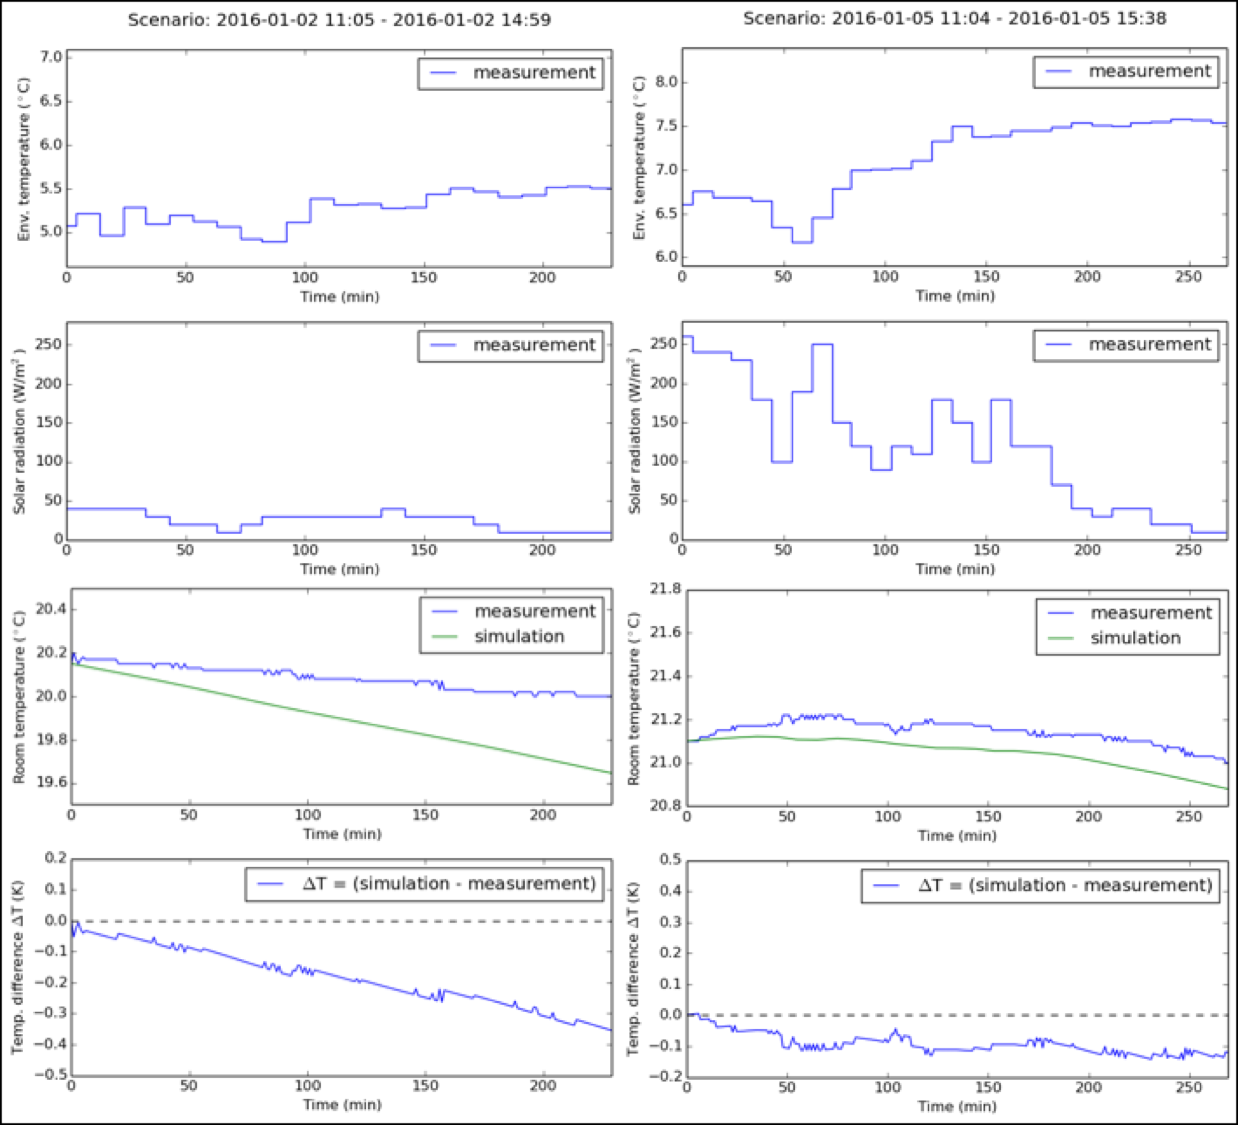
\includegraphics[width=\textwidth]{abbildungen/20160329_pestep2}
\caption{Parameterschätzung}
\label{fig:step2}
\end{figure}

Die Plots auf der linken Seite stellen das Ergebnis für ein 220-minütiges Intervall am 02.01.2016, auf der rechten Seite für ein 270 minütiges Intervall 05.01.2016 dar. Die Parameterschätzung ergab einen geschätzten Transmissionsgrad von $window_{transmission}=0.00687213$. Dieser Wert scheint zunächst unrealistisch klein. Bei einer genaueren Betrachtung ist zu beachten, dass wie bereits eingangs erwähnt bei der Parameterschätzung eine Anpassung des Modells an die Messwerte stattfindet, inklusive deren Störgrößen und Messfehler. Weiterhin ist der tatsächliche Transmissionsgrad der Fensterscheiben in K004b unbekannt, da der Fensterhersteller \textsc{Schüco} lediglich die Rahmen produziert. Das Unternehmen, welches die Glasscheiben eingesetzt und die Fenster montiert hat und damit die Information besitzt, konnte leider nicht ermittelt werden.

In den oberen Plots sind wiederum die Verläufe der Steuergrößen im Schätzintervall zu sehen. Die Außentemperaturen waren in beiden Intervallen mild zwischen fünf und acht Grad Celsius. im ersten Intervall wurde eine schwache, im zweiten hingegen wurde eine starke Globalstrahlung gemessen. Auf beiden Ergebnisplots ist zu erkennen, dass der Einfluss der Strahlung zum Ende des Intervalls hin immer weiter unterschätzt wird. Die Temperaturabweichung liegt bei beiden Intervallen unterhalb einem Betrag von $0,4^{\circ}C$. Im rechten Modellabgleich ist durch die leicht angedeuteten Senken sehr schön zu erkennen, dass das Verhalten des Modells mit der Realität trotz Abweichungen sehr gut abgebildet wird.
Unter der Berücksichtigung der Messfehler und da insbesondere die ersten Minuten der Simulation eine ausreichende Beschreibung der Realität liefern, sollte die Güte des Modells für eine Anwendung mit Modellprädiktiver Regelung ausreichen. 


Um die Verbesserung der Modellgüte einordnen zu können, erfolgt eine erneute Simulation des ersten Validierungsintervalls ohne den Einsatz eines Heizkörper. Die Ergebnisse sind im Plot in \ref{fig:valid1pe} dargestellt.

\begin{figure}
\centering
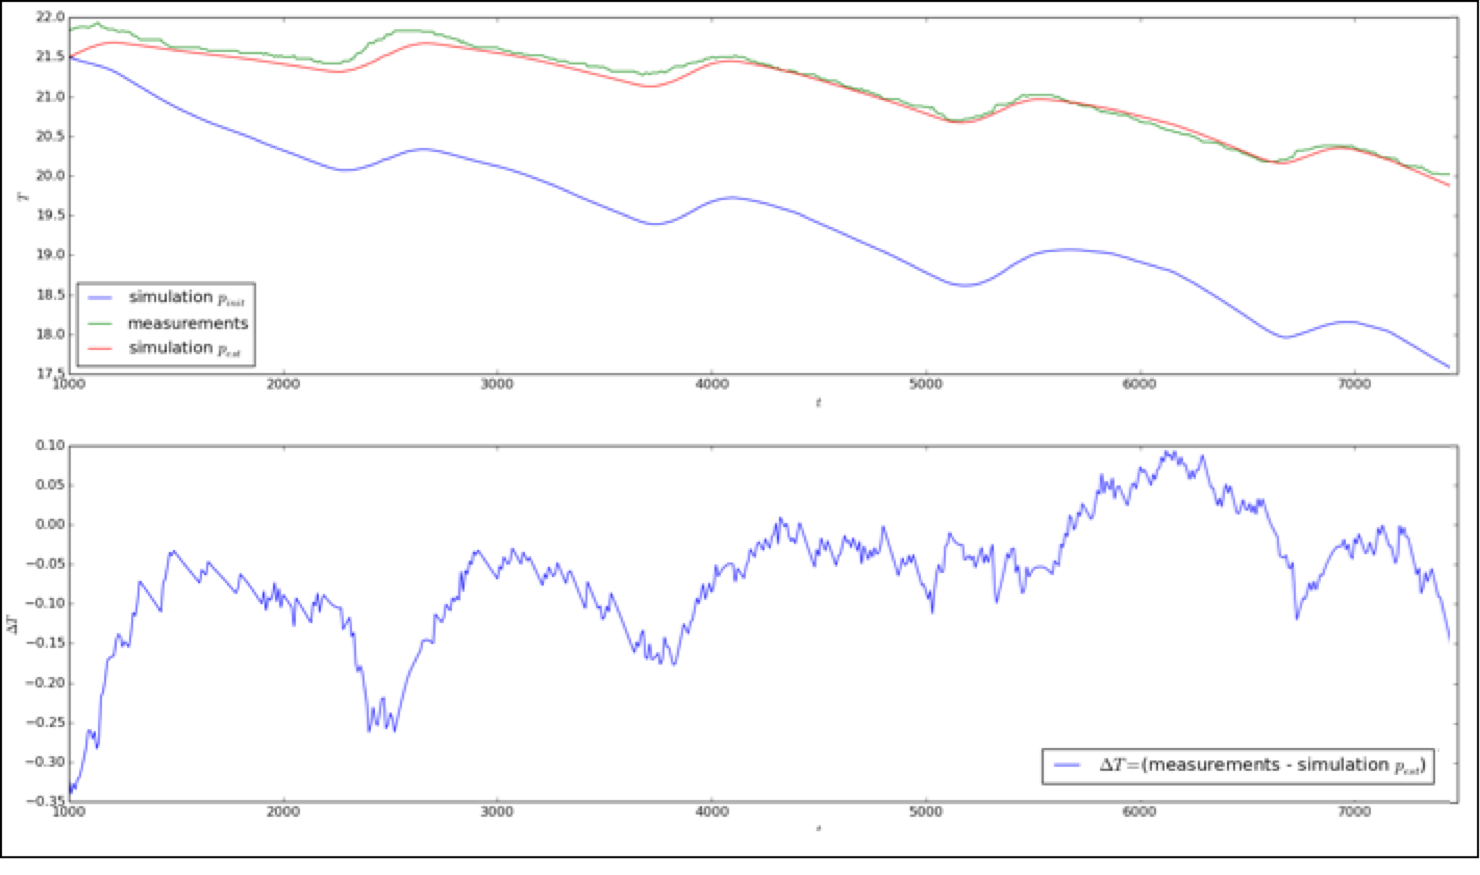
\includegraphics[width=\textwidth]{abbildungen/20160329_validierung1pe}
\caption{Simulation des Raummodells ohne Einsatz der Heizung mit geschätztem Parameter}
\label{fig:valid1pe}
\end{figure}

Abgesehen von einem Fehler bei der Initialisierung der Raumtemperatur zu Beginn der Simulation, ist eine erheblich Verbesserung zu erkennen. Über ein fünf-tägiges Intervall ist die Abweichung der Simulation sehr gering und die Dynamik des Systems wird sehr gut beschrieben.

Im letzen Schritt wird die Schätzung des Wärmedurchgangskoeffizienten des Heizkörpers durchgeführt. Es wurden Schätzintervalle identifiziert, an denen keine Solarstrahlung zu finden war und Störgrößen möglichst ausgeschlossen werden können. Dazu bieten sich zwei Intervalle am Abend des 17.01.2016, an dem die Heizung von der Anlage genutzt wurde. Die Ergebnisse der Parameterschätzung für die 20 Minuten umfassenden Intervalle sind in \ref{fig:step3} zusammengefasst. Das Skript zur Parameterschätzung findet sich im Anhang \ref{att:cd} in der Datei $room_pe_step3_radiator_night.py$.

\begin{figure}
\centering
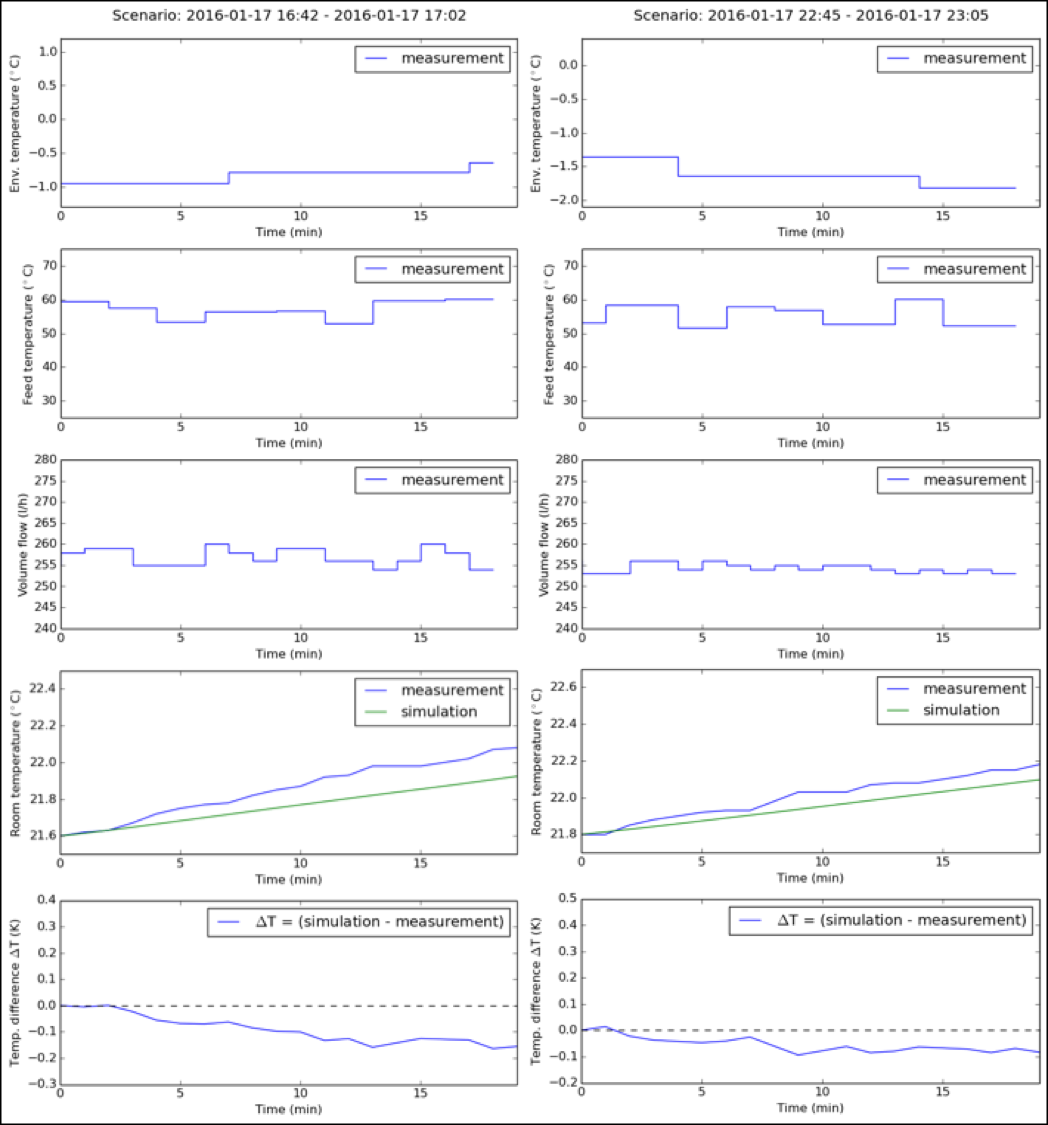
\includegraphics[width=\textwidth]{abbildungen/20160329_pestep3}
\caption{Parameterschätzung}
\label{fig:step3}
\end{figure}

Die Plots stellen das Ergebnis für die beiden 20-minütigen Intervalle dar. Die Parameterschätzung ergab einen realistischen Schätzwert für den Wärmedurchgangskoeffizienten des Heizkörpers von $u=_{radiator}=12.9872$.
Wie zuvor sind in den oberen Plots die Verläufe der Steuergrößen im Schätzintervall zu sehen. Die Außentemperaturen waren in beiden Intervallen knapp unterhalb des Gefrierpunkts und in keinem der beiden Intervalle wurde eine Globalstrahlung gemessen. Außerdem wurde die Heizung mit voller Leistung betrieben.
Auf beiden Ergebnisplots folgt die Simulation der Temperaturkurve sehr gut, wenn auch die Diskrepanz zum Ende des Intervalls hin zunimmt. Mit einer maximalen Temperaturabweichung bei beiden Intervallen mit einem Betrag von $0,2^{\circ}C$ beschreibt das Modell das reale Verhalten damit ausreichend.

Eine erneute Simulation des vorherigen Simulationsintervalls mit dem Einsatz des Heizkörper verdeutlicht eine Vrbesserung des Modells. Die Ergebnisse sind im Plot in \ref{fig:valid2pe} dargestellt.

\begin{figure}
\centering
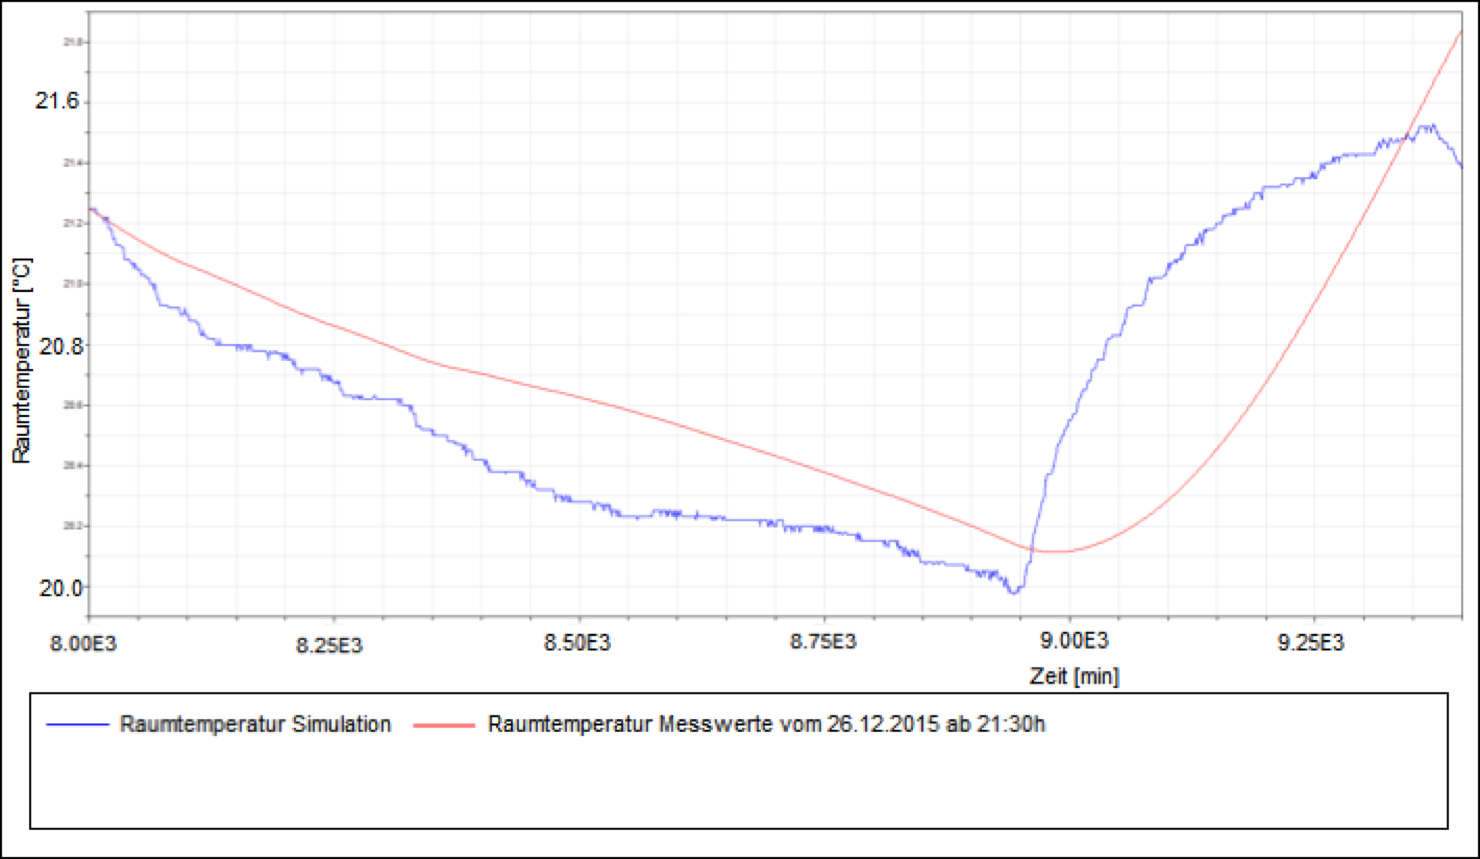
\includegraphics[width=\textwidth]{abbildungen/20160330_validierung2pe}
\caption{Simulation des Raummodells mit Einsatz des Heizkörpers mit geschätztem Parameter}
\label{fig:valid2pe}
\end{figure}

Die Abweichungen der Kurve sind deutlich verbessert sowie die Verzögerung hat sich verkürzt. Die Dynamik hat sich für das eintägige Intervall ebenfalls verbessert, wenn auch nur leicht.

Abschließend erfolgt eine Modellprädiktive Regelungsnahe Simulation des Modells. Das Ergebnis ist in \ref{fig:bench} dargestellt.

\begin{figure}
\centering
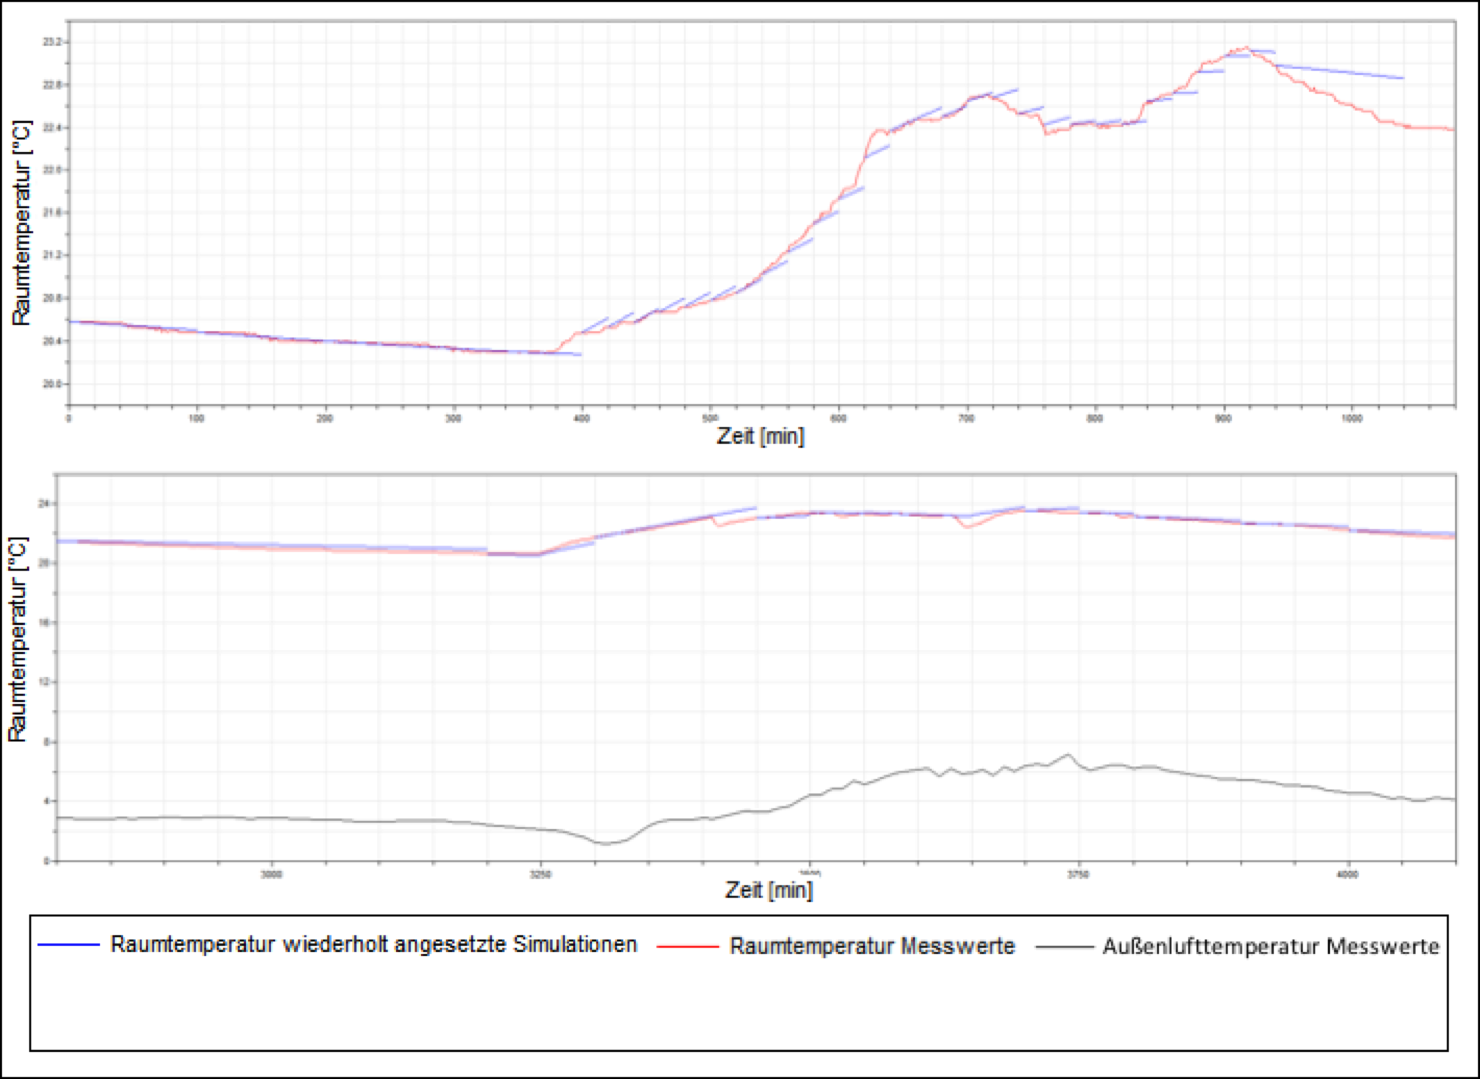
\includegraphics[width=\textwidth]{abbildungen/20160330_benchmark}
\caption{Simulation des Raummodells mit Einsatz des Heizkörpers mit geschätztem Parameter}
\label{fig:bench}
\end{figure}

Es wurden wiederholt kürzere Simulationen mit einer angepassten Initialtemperatur angesetzt, um eine Struktur ähnlich der Modellprädiktiven Regelung zu erhalten. Die Außenlufttemperatur bewegte sich während des Zeitraums knapp über dem Gefrierpunkt und es wurde lediglich eine schwache Globalstrahlung detektiert. Beim Einsatz der Heizung wurden kürzere Simulationsintervalle von 20 Minuten angesetzt, ansonsten wurden die Simulationen für längere Intervalle durchgeführt.
Nach 800 simulierten Minuten setzt die Heizung ein, was durch das Modell gut abgebildet wird. Es bestehen lediglich Abweichungen an zwei kleineren Abfällen der gemessenen Temperatur, die sich durch Störgrößen wie beispielsweise das Öffnen der Fenster erklären lassen, und daher vom Modell nicht berücksichtigt wurden.

Zusammenfassend lässt sich feststellen, dass das Modell eine solide Beschreibung des Verhaltens von K004b darstellt und sich damit für den Einsatz in der \acrlong{mpr} eignet. Im letzten Abschnitt wird überprüft, ob das Modell den Anforderungen für den Einsatz mit \textsc{JModelica.org} genügt.

\section{Modellprädiktive Regelung}

Um eine \acrlong{mpr} in \textsc{\textsc{JModelica.org}} anhand des Raummodells zu ermöglichen, wird das Modell in ein Optimierungsfähiges Objekt übersetzt. Dazu wird das Modell mithilfe des \textsc{JModelica.org} Compilers in ein JMU und Optimization Object transferiert anhand des Programms in Listing \ref{lst:comp}.

\lstinputlisting[language=Python ,caption={Programm zur Übersetzung des Raummodells in Optimierungsfähige Objekte in \textsc{JModelica.org}}, label=lst:comp]{listings/compiling.py}

Trotz der Ausgabe von kleineren Warnungen, lässt sich das Modell übersetzen und damit für Optimierungszwecke in \textsc{JModelica.org}nutzen. Eine Bestätigung in der Python Konsole für das erfolgreich übersetzte Problem findet sich in \ref{fig:jmod}.

\begin{figure}
\centering
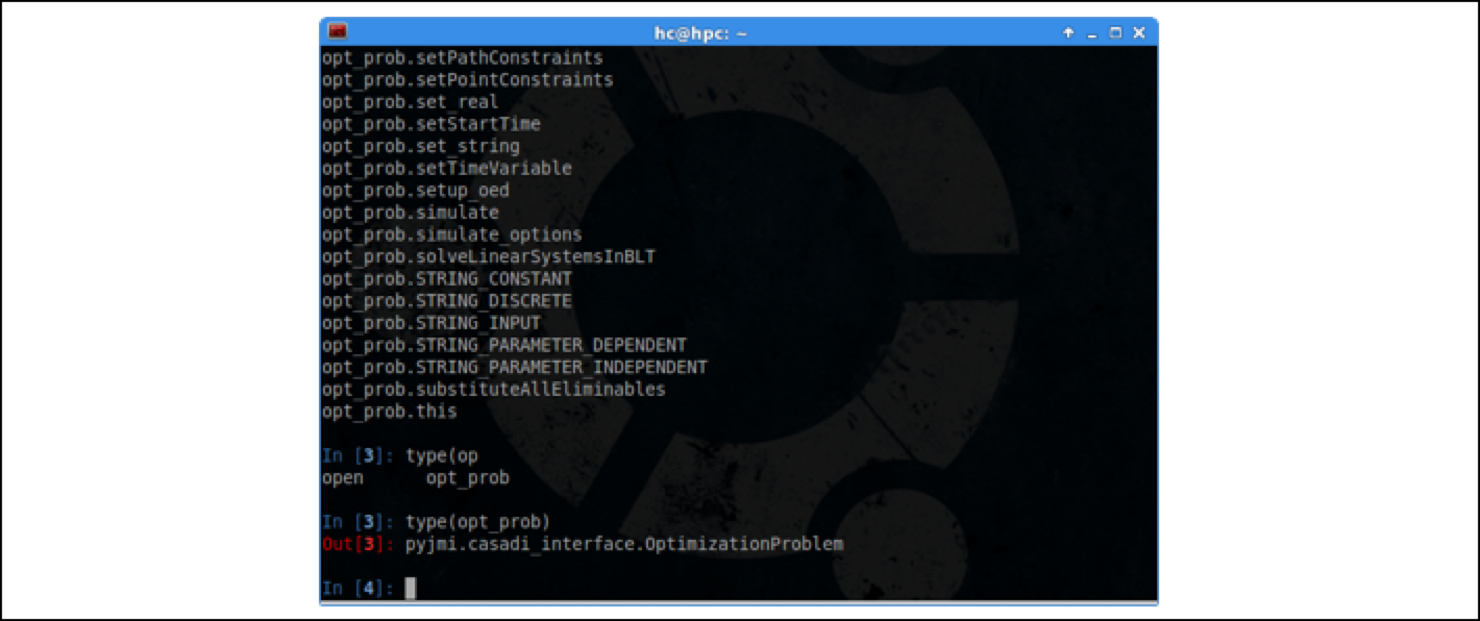
\includegraphics[width=\textwidth]{abbildungen/20160330_mpc}
\caption{\textsc{\textsc{JModelica.org}} Kompabiltät des Modells}
\label{fig:jmod}
\end{figure}

Die Hypothese, dass sich das Modell für den Einsatz mit \textsc{JModelica.org} eignet, kann also bestätigt werden.
Damit sind die Voraussetzungen für eine Modellprädiktive Regelung der Raumtemperatur in K004b geschaffen.